\begin{frame}[t]
  \frametitle{Introduction}
  \begin{columns}
    \begin{column}{0.6\textwidth}
    Imagine our solar system...
    
    \vspace{1em}
    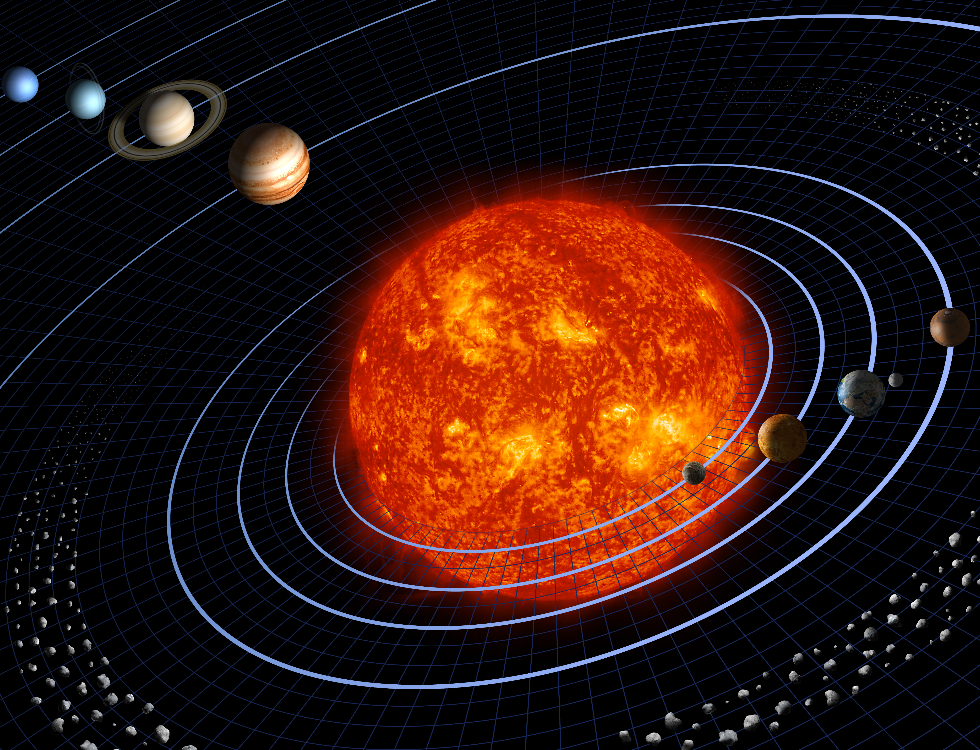
\includegraphics[width=\textwidth]{solar} \\
    \scriptsize (Image from NASA)
    \end{column}
    \begin{column}{0.35\textwidth}
      \centering
      $\vec{F} = m\vec{a}$
      \begin{alignat*}{3}
      & \text{Mercury:} \quad && \vec{r}_1(t) \\
      & \text{Venus:}   \quad && \vec{r}_2(t) \\
      & \text{Earth:}   \quad && \vec{r}_3(t) \\
      & \text{Mars:}    \quad && \vec{r}_4(t) \\
      & && \vdots
      \end{alignat*}
      \pause Analytical solution: \alert{$\textrm{\ding{55}}$} \\
      Numerical solution: \emph{$\textrm{\ding{51}}$}
    \end{column}
  \end{columns}
\end{frame}

\begin{frame}[t]
  \frametitle{Introduction}
  \begin{columns}
    \begin{column}{0.35\textwidth}
    \makebox{Scaling down to $10^{-10}$ meters...}
    
    \vspace{1em}
    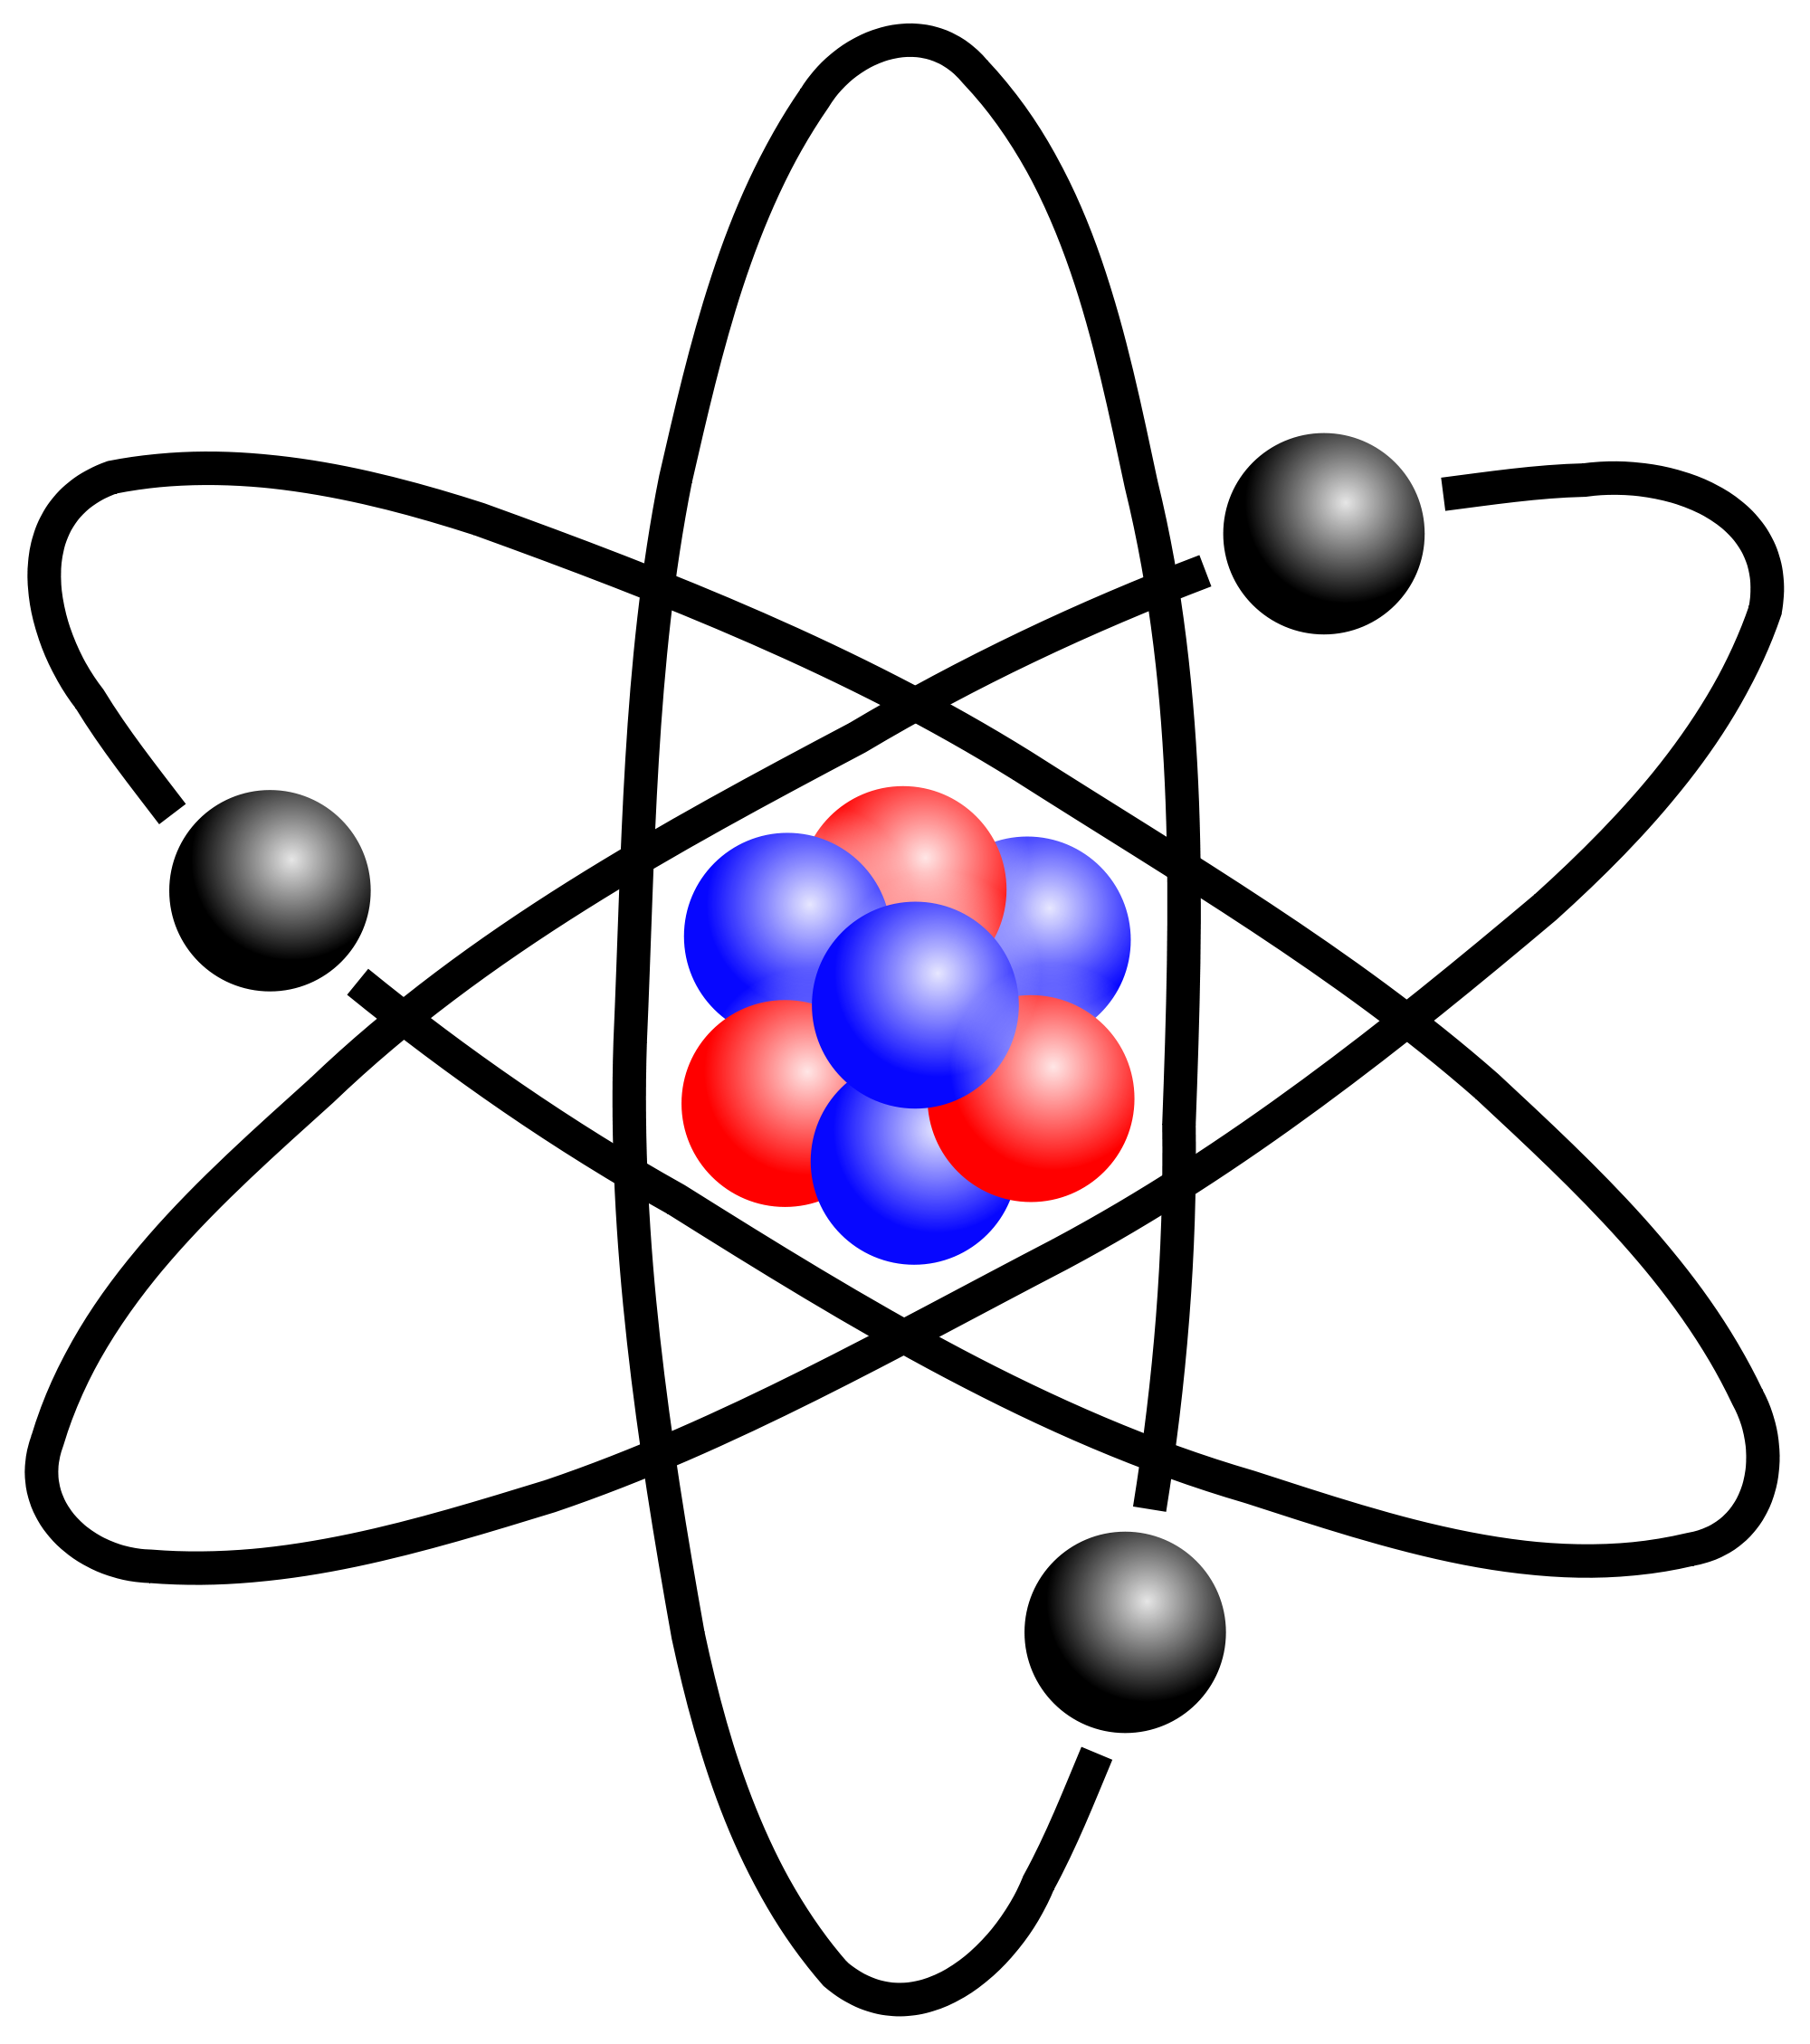
\includegraphics[width=\textwidth]{atom} \\
    \scriptsize (Image from Wikipedia)
    \end{column}
    \begin{column}{0.6\textwidth}
      \[H \Psi = E \Psi\]
      \[H = \sum_{i=1}^N \left[ -\frac{1}{2} \nabla_i^2 - \frac{Z}{r_i} \right] + \sum_{i<j}^N \frac{1}{|\vec{r}_i - \vec{r}_j|}\]
      \centering
      Many-electron wave function
      \[\Psi(\vec{r}_1,\vec{r}_2,\ldots,\vec{r}_N)\]
      
      \pause Analytical solution: \alert{$\textrm{\ding{55}}$} \\
      Numerical solution: \alert{$\textrm{\ding{55}}$}
      
      \vspace{1em}
      \pause \emph{$\boxed{\text{Approximations!}}$}
    \end{column}
  \end{columns}
\end{frame}


